\section{Exploratory Analysis} \label{explore}
We wanted to first see if LDA and QDA were potential models by checking for normal covariates.  We saw that there were a large number of factors in the data, and so we tried only considering the numerical predictors, and used histograms to see if we could rule out normal distributions.  These are shown in Figure \ref{fig:NonNormalHists}.  It is clear that all of these are far from being able to be assumed to follow normal distributions, and thus we presume that LDA and QDA models are not appropriate and would not yield predictive models.

\begin{figure}[h]
    \centering
    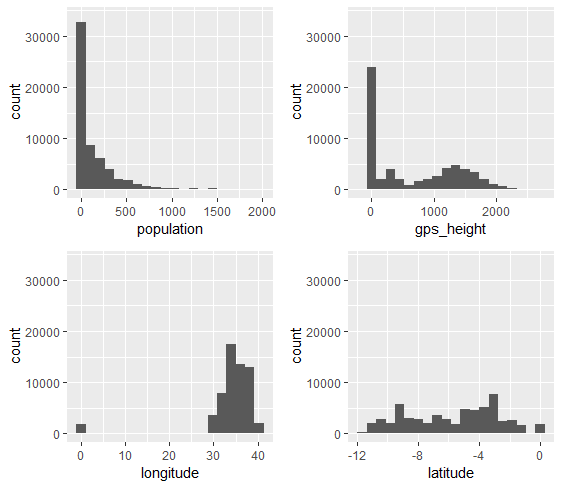
\includegraphics[width=0.6\textwidth]{Figures/HistsNotNormal.png}
    \caption{Histograms of some of the numerical predictors.}
    \label{fig:NonNormalHists}
\end{figure}